\documentclass [11pt,twoside]{report}  % Página A4, usa ambos os lados da folha 
\usepackage[utf8]{inputenc}
\usepackage{graphicx}
\usepackage[a4paper, width=150mm, top=25mm, bottom=25mm, bindingoffset=6mm]{geometry}
\setcounter{tocdepth}{3}
\setcounter{secnumdepth}{3}
\usepackage{float}
\usepackage[toc,page]{appendix}
\usepackage{subcaption}

\usepackage{acronym} 

\usepackage{helvet}  % usar Arial para o documento inteiro
\renewcommand{\familydefault}{\sfdefault}

% biber
\usepackage[backend=biber, style=ieee, url=true]{biblatex}
\addbibresource{ref.bib}

\usepackage{amsmath}  	%equacoes
\usepackage{amsfonts}	%equacoes

%\usepackage{tikz} %riscos

%\usepackage{rotating}%rodar texto

% Checkmark
%\usepackage{bbding}

% Tabela das equações 
%\usepackage{tabularx}

% cores das tabelas
%\usepackage[table,xcdraw]{xcolor}

% Font
%\usepackage{fontspec}
%\setmainfont{Times New Roman}

% Imagens Separadas
%\usepackage{subcaption}

% Numeracao Romana
%\usepackage{array}

\usepackage{listings}
\usepackage{color}




% Highlight Paragraph
\usepackage[most]{tcolorbox}

\newtcbox{\hl}{
  on line,
  colback=yellow!80,
  colframe=white,
  boxrule=0pt,
  arc=0pt,
  boxsep=1pt,
  left=0pt,
  right=0pt,
  top=0pt,
  bottom=0pt
}
\captionsetup[subfigure]{list=true}


\begin{document}
%--------------------------------------------------------------------------------------------------------- CAPA
\thispagestyle{empty}
\begin{center}
\begin{figure}[H]
  	\centering   
    
\includegraphics[width=10cm]{imagens/logo_isel.png}
\end{figure}


%Título do Projecto 

\vspace{40mm}

\LARGE\textbf{
Modular Platform for Data Acquisition and Analysis Based on CAN for Distributed Vehicular Systems
}\\

\vspace*{\fill}

%NOME DO CANDIDATO
\Large Luís Henrique Ferreira\\
\Large Gonçalo José Ferraz\\

\vspace{10mm} 

%Tipo de Trabalho 
\fontsize{10pt}{10pt}\selectfont
Project in the Field of Computer and Informatics Engineering


\vspace{10mm} 

\large{Supervisors:}\\
\normalsize
Eng. David Emanuel Ribeiro Velez\\

\vspace{10mm}  

\large{Jury:}\\
\normalsize
President: Doctor Fernando Sousa\\
Vowels:
Doctor Rui Duarte\\
Eng. David Emanuel Ribeiro Velez\\

\vspace{10mm} 

\small\textbf{July of 2026}
\normalsize
\end{center}
\newpage
\thispagestyle{empty}
\textbf{}
\clearpage

%--------------------------------------------------------------------------------------------------------- Página de rosto
\thispagestyle{empty}
\begin{figure}[H]
  	\centering   
    
\includegraphics[width=10cm]{imagens/logo_isel.png}
\end{figure}

\vspace{40mm}
\begin{center}
%Título do Projecto 

\LARGE\textbf{Modular Platform for Data Acquisition and Analysis Based on CAN for Distributed Vehicular Systems}\\

\vspace*{\fill}

%NOME DO CANDIDATO
\Large Luís Henrique Ferreira\\
\Large Gonçalo José Ferraz\\

\vspace{10mm} 

%Tipo de Trabalho 
\fontsize{10pt}{10pt}\selectfont
Project in the Field of Computer and Informatics Engineering


\vspace{10mm} 

\large{Supervisors:}\\
\normalsize
Eng. David Emanuel Ribeiro Velez\\

\vspace{10mm} 

\large{Jury:}\\
\normalsize
President: Doctor Fernando Sousa\\
Vowels:
Doctor Rui Duarte\\
Eng. David Emanuel Ribeiro Velez\\


\vspace{10mm} 

\small\textbf{July of 2026}
\normalsize


\end{center}
\clearpage
\thispagestyle{empty}
\textbf{}
\clearpage
%----------------------------------- AI disclosure

\vspace*{\fill}
\begin{center}
\subsection*{AI usage disclosure}
\end{center}

In this project we utilized AI modules in order to research and assist with the development, more specifically in the context of:
\vspace{10mm}
\begin{center}
    Bluetooth Integration with BlueZ Framework Research
    \par
    Android UI Presentation
    \par
    CAN Decoding
    \par
\end{center}
\vspace*{\fill}

\clearpage


%----------------------------------- Statement of Integrity

\vspace*{\fill}
\begin{center}
\subsection*{Statement of Integrity}
\end{center}

I declare that this project work is the result of my personal
and independent research. Its content is original, and all sources listed in the bibliographic references
were consulted and are duly mentioned in the text. I further declare that all scientific and technical
references relevant to the development of the work are duly cited and included in the bibliographic
references.

\vspace{10mm}

\begin{center}
    The authors
\end{center}

\begin{center}
    Luís Henrique Borges Coury Cavaleiro de Ferreira
    \par
    Gonçalo José Soeiro Ferraz
    \par
\end{center}
\vspace*{\fill}
\clearpage

%-----------------------------------
\pagenumbering{roman}		% Numeração Romana 

% Indice
\tableofcontents 
% Lista de Tabelas
\listoftables
% Lista de Figuras
\listoffigures

% Lista de Acrónimos
\chapter*{List of Acronyms}		% use \ac{*}
\begin{acronym}[MPC] % Give the longest label here so that the list is nicely aligned
\acro{ADV}{Ignition Advance}
\acro{AFR}{Air-Fuel Ratio}
\acro{API}{Application Programming Interface}
\acro{BCU}{Battery Unit Control}
\acro{BLE}{Bluetooth Low-Energy}
\acro{CAN}{Controller Area Network}
\acro{CLT}{Coolant Temperature}
\acro{CPU}{Central Processing Unit}
\acro{CRC}{Cyclic Redundancy Check}
\acro{DB}{Database}
\acro{ECU}{Electronic Control Unit}
\acro{EGO}{Exhaust Gas Oxygen}
\acro{EV}{Eletric Vehicle}
\acro{FP}{Fuel Pump}
\acro{GATT}{Generic Attribute Profile}
\acro{GPIO}{General Purpose Input/Output}
\acro{GUI}{Graphical User Interface}
\acro{IAT}{Intake Air Temperature}
\acro{ICE}{Internal Combustion Engine}
\acro{JSON}{JavaScript Object Notation}
\acro{MAP}{Manifold Absolute Pressure}
\acro{PWM}{Pulse Width Modulation}
\acro{RAM}{Random Access Memory}
\acro{RPM}{Revolutions Per Minute}
\acro{RT}{Real-Time}
\acro{SQL}{Structured Query Language}
\acro{SoC}{System on Chip}
\acro{TPS}{Throttle Position Sensor}
\acro{UART}{Universal Asynchronous Receiver-Transmitter}
\acro{USB}{Universal Serial Bus}
\acro{UUID}{Universally Unique Identifier}
\acro{VCU}{Vehicle Control Unit}
\acro{VSS}{Vehicle Speed Sensor}
\acro{VE}{Volumetric Efficiency}
\end{acronym}		
\clearpage 

%-----------------------------------
\pagenumbering{arabic}		% Numeração Arábica 
%\setcounter{chapter}{0}

\chapter{Introduction}

\hspace{5mm} The document describes the development of a modular data acquisition and analysis platform based on Controller Area Network (CAN) communication, designed for application in distributed vehicular systems. Modern vehicles exhibit increasing electronic complexity and a high distribution of control units and sensors, making it essential to provide tools and solutions capable of centralizing, interpreting, and exploring data efficiently. This project proposes an integrated approach that combines real-time data acquisition, structured storage, and analysis and visualization tools, with the objective of improving the understanding of vehicle behavior and supporting technical decision-making processes in demanding environments such as motorsport.


\section{Context and Framework}

This project is developed within the scope of the Project and Seminar curricular unit of the Bachelor's Degree in Computer and Informatics Engineering (LEIC) at Instituto Superior de Engenharia de Lisboa, during the 2025/2026 academic year. The project’s application domain focuses on distributed vehicular systems, with particular emphasis on the Motorsport and aftermarket sectors. These contexts are characterized by demanding requirements in terms of real-time data acquisition, transmission, and analysis, which are essential for performance monitoring, fault diagnosis, and system optimization. The increasing electronic complexity and the vast diversity of systems used in modern vehicles and/or motorsport/enthusiast applications make the development of modular, flexible, and scalable platforms essential.

The platform is developed based on the Raspberry Pi ecosystem, taking advantage of its versatility, low cost, and extensive support documentation. The project primarily uses the \textit{Python} and \textit{Bash} programming languages, enabling a hybrid approach that combines ease of development with execution capability in embedded systems. This technological choice aims to facilitate rapid prototyping while ensuring flexibility for adaptation to different usage scenarios.

A distinguishing element of this project is its validation environment, which takes place in the real-world context of a vehicle equipped with a \textit{RusEFI} ECU, as well as within a Formula Student project. This framework allows not only the testing of the solution under conditions close to real operation, but also dealing with practical challenges such as hardware constraints, electromagnetic noise, communication limitations, and robustness and reliability requirements. Integration into a competition vehicle also adds a critical real-time and performance dimension, where data-driven decisions can have a direct impact on achieved results.

In summary, this project is positioned at the intersection of software engineering and embedded systems applied to the automotive domain, seeking to address the growing need for modular and efficient solutions for data acquisition and analysis in distributed vehicular systems.\\


\section{Problem and Motivation}

The development of modern vehicular systems raises a set of significant challenges regarding data acquisition, integration, and interpretation. One of the main identified issues is the strong dependence on the vehicle’s Electronic Control Units (ECUs), which often operate as closed systems, limiting direct and flexible access to information. In this context, the need arises to create an autonomous and fully parameterizable solution capable of ensuring independence from these units, with the objective of enabling the integration of different applications through database access via Bluetooth. The use of CAN databases (DBC) plays a central role in this approach, allowing the structured decoding and interpretation of messages without requiring direct intervention in the ECUs.

At the same time, the increasing complexity of distributed vehicular systems introduces additional challenges in data management. In a modern vehicle, multiple subsystems coexist, such as the ECU, VCU (Vehicle Control Unit), and BCU (Battery Control Unit), each responsible for different critical functions. These subsystems often communicate through different protocols, such as CAN, serial communication, Wi-Fi, or Bluetooth, resulting in a heterogeneous and fragmented ecosystem. The absence of a unifying platform makes the centralization and synchronization of information difficult, compromising its practical usefulness.

In competitive environments such as Formula Student, this data fragmentation translates into a concrete limitation: the difficulty of correlating information originating from different sources. Without robust integrated analysis tools, it becomes challenging to identify performance patterns, understand the vehicle’s dynamic behavior, or detect anomalies in a timely manner. This limitation may have a direct impact on the vehicle optimization process, reducing the effectiveness of the technical decisions made by the team.

Thus, the central motivation of the project lies in the creation of a distributed platform capable of simultaneously transforming large volumes of raw data into structured, clear, actionable, and persistent information. The goal is not only to collect data, but also to provide tools that enable its efficient analysis and interpretation. By facilitating the visualization, correlation, and processing of information, the proposed solution aims to support more informed decision-making, contributing to the continuous improvement of the performance and reliability of vehicular systems.

\section{Objectives}

This project establishes clearly defined objectives, with success assessed through tangible, result-oriented outcomes, culminating in the development and real-world validation of a functional platform:

\begin{itemize}

\item \textbf{Design a modular and scalable architecture}, that facilitates the integration of the platform to different vehicles, sensors, and technical requirements, minimizing the need for structural changes to the system.

\item \textbf{Develop a CAN-based data acquisition system}, with the ability to decode messages using DBC files, ensuring reliable real-time reading of relevant vehicle signals.

\item \textbf{Create an efficient and continuous data logging system}, enabling structured recording of data during extended sessions, without information loss and with guarantees of integrity. Develop a modular real-time dashboard for data visualization, allowing monitoring of critical vehicle parameters with low latency and high clarity, and configurable according to the use context.

\item \textbf{Implement a multichannel data integration mechanism},  capable of aggregating information from different subsystems and protocols (CAN, UART, and Bluetooth), ensuring consistent time synchronization between sources.

\item \textbf{Implement data analysis tools}, including statistical analysis methods, session comparison, and anomaly detection, with the aim of extracting relevant information from the collected data.

\item \textbf{Ensure system robustness and reliability}, guaranteeing stable operation in demanding environments subject to noise, vibration, and power fluctuations. Validate the solution in a real environment through its integration into a vehicle within a Formula Student context, demonstrating its practical applicability and performance under operational conditions.

\end{itemize}


\section{Document Structure}

This document is structured to demonstrate an understanding of the research conducted, the necessary knowledge for its comprehension, the proposed solution, and the results obtained. More specifically:

\begin{itemize}
    \item \textbf{Chapter 2 - State of the Art:} Reviews the necessary knowledge for the proper interpretation of the thesis, from the inner-workings of a  controller area network and how their vehicular information is revealed,  the process and analysis of the sensor information to the bluetooth information transfer protocols
    \item \textbf{Chapter 3 - Implementation:} Details of the design choices, experimental setup, system and database architecture and data analysis 
    \item \textbf{Chapter 4 - Results and Validation:} Experimental results of the project, detailing the experimental environment and the results given
    \item \textbf{Chapter 5 - Conclusion:} Final thoughts about the project design and implementation and future possible changes to better optimize and develop the project
\end{itemize}





\chapter{State of the Art}


\hspace{5mm} Modern vehicles rely on a distributed electronic architecture composed of multiple interconnected control systems that continuously monitor and manage vehicle operation. At the core of this architecture are ECUs, which process data from numerous sensors and coordinate the operation of vehicle subsystems to ensure optimal performance, efficiency, safety, and compliance with regulatory requirements. ECUs are responsible for controlling engine sensors and actuators, as well as providing various vehicle operating parameters such as engine speed (RPM), pressures, temperatures, air-fuel mixture, and other relevant indicators \cite{jg}.



\section{Vehicular Communication Networks}

\subsection{Electronic Control Unit}

It functions as a small embedded computer, acquiring information from sensors, processing this data in real time, and sending commands to actuators. Depending on its purpose, an ECU may control the engine, transmission, ABS braking system, stability control, power steering, airbags, and many other systems found in modern automobiles \cite{jg}.

The development of ECUs became increasingly relevant during the 1970s and 1980s, driven by the need to improve engine efficiency and reduce pollutant emissions. 

Before the development of ECU, automotive systems were mostly mechanical. As vehicles became more a more complex and had more stict regulations, there was a need for more precise electronic solutions, leading to the creation of the first ECUs


\subsection{Controller Area Network}


The \ac{CAN} Network is a vehicle message-based communication protocol design to allow an ECU to communicate to other devices without the need for a central computer and to enable a fast and reliable exchange of information between electronic modules \cite{iso11898}. 

This protocol was developed by Robert Bosch GmbH in the 1980s as a response to the increasing complex vehicular systems of the time. Over time, the CAN protocol became the standard due to it's simplicity and ability to operate in electrically noisy environment.

\begin{figure}[H]
  	\centering   
    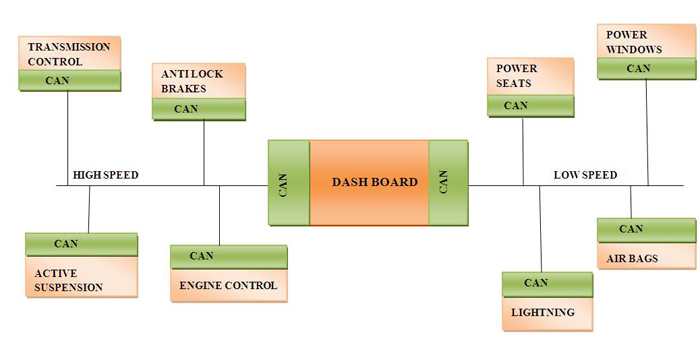
\includegraphics[width=0.8\linewidth]{imagens/Can_protocol.png}
    \caption{CAN Application Example \cite{canprotocol}}
    \label{fig:prj_arch}
\end{figure}

CAN protocol is a message-based protocol. This means the data of a vehicule is transmitted in messages identified by a unique ID and available for every electronic module to read, instead of being sent to specific devices. Any ECU on the network can broadcast messages, and any other ECU can choose to listen to the messages relevant to it.

These messages, known as frame, follow a specific format as to ensure consistency:
\begin{itemize}
    \item ID - Unique message identifier
    \item DLC (Data Length Code) - Specifies the data length in bytes
    \item Data Field - Contain the information payload 
    \item CRC (Cyclic Redundancy Check) - Used for error and data integrity verification
    \item ACK Slot - Confirms reception of at least one node
    \item EOF (End of Frame) - Signals the end of the message
\end{itemize}

\begin{figure}[H]
  	\centering   
    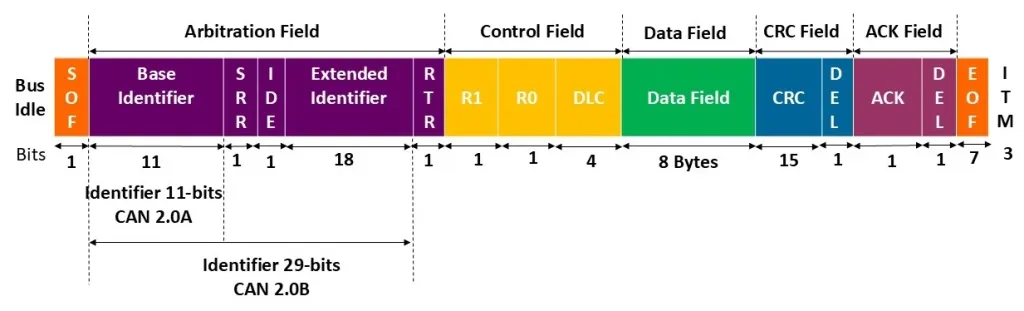
\includegraphics[width=1\linewidth]{imagens/CAN-Protocol-Extended-Frame-Format.png}
    \caption{CAN Standard Data Frame \cite{canframe}}
    \label{fig:prj_arch}
\end{figure}


\subsection{Controller Area Network Data Base}

CAN databases, commonly represented as DBC files, play a fundamental role in the interpretation and use of CAN bus data in modern automotive and embedded systems. A CAN database defines the structure and semantics of CAN messages, enabling the translation of raw binary frames into meaningful physical signals.
A CAN frame, by itself, only contains an identifier and a sequence of data bytes. Without additional context, this data is not directly interpretable. CAN databases address this limitation by providing a structured description of each message, including its identifier, length, and the layout of individual signals within the payload. Each signal is defined through parameters such as bit position, bit length, scaling factor, offset, and engineering units. This makes it possible to convert raw byte streams into values such as engine speed in revolutions per minute, throttle position, or air fuel ratio \cite{vectorcandb}. 
One of the primary use cases of CAN databases is real-time data decoding. In systems such as ECU monitoring platforms or vehicle telemetry applications, incoming CAN frames are matched against database definitions and decoded into structured data. This enables the development of dashboards, logging systems, and diagnostic tools that present meaningful information to the user. In the context of the proposed solution, the DBC file is used to decode messages from a rusefi ECU, translating low level CAN frames into a normalized vehicle state.
Another relevant application is data logging and offline analysis. CAN databases allow raw CAN traffic to be recorded while preserving the ability to decode it at a later stage. This is particularly useful for debugging, performance evaluation, and research activities. Since decoding logic is defined externally in the database, previously recorded data can be reinterpreted using updated signal definitions without requiring any modification to the stored dataset.
CAN databases are also widely used in simulation and testing environments. By defining message structures and signal properties, DBC files allow synthetic CAN traffic to be generated in a controlled manner. This capability is important in hardware in the loop and software validation scenarios, where realistic communication patterns are required without relying on physical ECUs.
Additionally, DBC files contribute to standardization and interoperability across different tools and systems. Multiple applications such as CAN analyzers, embedded controllers, and data acquisition platforms can use the same database to ensure consistent interpretation of CAN messages. This reduces ambiguity and simplifies integration in complex systems involving multiple components and suppliers \cite{pfeiffer}.

\subsection{Why CAN is the Preferred Method for Intra-Vehicular Communication}

Controller Area Network (CAN) is widely adopted in intra-vehicular communication due to its deterministic behavior, fault tolerance, and efficient bus architecture. It is specifically designed for distributed embedded systems where multiple ECUs must exchange time-critical information over a shared medium \cite{bosch}.

CAN employs a multi-master, message-oriented communication model over a differential two-wire bus, which increases noise immunity in electrically harsh automotive environments. Reliability is ensured through multiple built-in mechanisms, including CRC, bit stuffing, frame validation, and automatic retransmission upon error detection. Fault confinement is also supported, allowing malfunctioning nodes to be isolated from the network.

A key feature of CAN is its non-destructive bitwise arbitration mechanism, which guarantees deterministic access to the bus. Message priority is encoded in the identifier field, where lower numerical values correspond to higher priority. During arbitration, nodes transmit simultaneously and monitor the bus, withdrawing transmission if a dominant bit is overwritten by a recessive bit. This ensures that the highest priority message is transmitted without collision or delay.

In terms of efficiency, CAN minimizes wiring complexity by using a shared bus topology, reducing both system cost and physical weight. It supports data rates up to 1 Mbps in Classical CAN, which is sufficient for most control applications. The protocol also allows both 11-bit and 29-bit identifiers, enabling flexible message addressing schemes, as shown in Figure 2.2.

\subsection{Standalone ECU}

Standalone ECUs are aftermarket electronic control systems designed to fully replace the original equipment manufacturer (OEM) ECU. Their primary purpose is to provide greater flexibility, configurability, and control over engine operation, particularly in high-performance and motorsport applications.

Unlike OEM ECUs, which are typically optimized for emissions, reliability, and mass production constraints, standalone ECUs allow direct access to key engine parameters such as fuel injection, ignition timing, boost control, and sensor calibration. This enables precise tuning of engine behaviour according to specific requirements, such as performance optimization, component modifications, or experimental configurations.

The motivation for using standalone ECUs arises from the need for adaptability and transparency. In applications such as Formula Student, where vehicles are custom-built and continuously refined, engineers require full control over the engine management strategy. Standalone ECUs provide this capability by supporting user-defined maps, real-time parameter adjustment, and integration with external systems through communication protocols such as CAN.

\subsection{Speeduino/RusEFI ECUs}

Speeduino and RusEFI are open-source standalone ECU platforms designed to provide flexible and low-cost engine management solutions. Both systems aim to replicate and extend the functionality of commercial standalone ECUs, while maintaining full transparency and user control over hardware and software \cite{rusefi_website}.

Speeduino is based on Arduino-compatible hardware and focuses on simplicity and accessibility. It provides core engine control features such as fuel injection, ignition timing, and sensor processing, making it a popular choice for educational projects and low-budget motorsport applications. Its architecture allows easy integration with existing tools such as TunerStudio, enabling real-time tuning and data logging.

RusEFI, on the other hand, targets more advanced use cases with a higher level of performance and configurability. It typically runs on more powerful microcontrollers and offers extended features, including native CAN support, higher processing capabilities, and more precise control strategies. This makes it suitable for more demanding applications, such as competitive motorsport or complex engine setups \cite{rusefi_github}.

The main motivation behind both platforms is to provide open, customizable alternatives to proprietary ECUs. They allow users to modify control algorithms, extend communication interfaces, and integrate telemetry systems, such as the one proposed in this work. As a result, they are particularly well suited for environments like Formula Student, where flexibility, experimentation, and cost constraints are critical factors.

\section{Embedded System's Development Platforms}

\subsection{Raspberry Pi Ecosystem}

For the controller of our project, we decide to utilize a Raspberry Pi Zero 2W \cite{raspizero2w}. This decision was made due to several reasons:
\begin{itemize}
    \item \textbf{Full Linux Computer:} The controller will have to implement several different tasks at once such as:
    \begin{itemize}
        \item Real-time data aquisition from the ECU
        \item Data processing like filtering and parsing signals
        \item Database logging and managment
        \item UI rendering
        \item Real-time bluetooth data transfer
    \end{itemize}
    A Raspberry Pi system provides a good flexibility to develop our application while being able to build our application with the features above.
    \item\textbf{Fast processor and decent memory:}
    The Raspberry Pi Zero 2 W incorporates a quad-core 64-bit Arm Cortex-A53 CPU clocked at 1GHz, paired with 512MB of LPDDR2 SDRAM. This package provides the Raspberry Pi Zero 2 W with good performance for our application, and having multiple cores will help with our distributed system aproach.
    
    \item \textbf{Easy communication with hardware:} The Raspberry Pi provides a USB serial port with the possibility to use UART pins already built-in to the computer
    \item \textbf{Networking:} This computer provides a Bluetooth Low Energy (BLE) system which allows the transfer of the CAN signal information easily to a connected mobile device
\end{itemize}

With all this said, we choose the Raspberry Pi for its fast performance, and affordable price. Another deciding factor in the selection of this computer was the extensive community support, along with the large number of available open-source projects and software resources.


\subsection{Utilized Programming Languages}

Support for multiple programming languages was a key design consideration, allowing each component to leverage the strengths of the most appropriate language while mitigating its inherent limitations:
\begin{itemize}
    \item \textbf{Python:} Used for the controller application for a ECU data pipeline, controller logic and bluetooth integration due to it's simplicity for serial communication, data parsing and bluetooth features as well as extensive UI libraries;
    \item \textbf{SQLite:} Although Python is used for making requests to the database, said requests are in SQL using a SQLite variant due to being a light-weight alternative to variants like Postgres, for the simplicity of easy for there is no need for a database and instead SQLite stores information in a single file and has extremely fast writes which is perfect for storing the CAN dataframes obtained;
    \item \textbf{Kotlin:} Kotlin was chosen as the primary language for mobile application development due to its seamless integration with the Android platform, support for low-latency applications, comprehensive networking libraries, and the modern Jetpack Compose UI framework.
\end{itemize}


\section{Data Analysis Techniques in Motorsport}
\subsection{Statistical Analysis}

The data gathered by the ECU enables a wide range of analytical applications, including engine tuning, performance evaluation in track environments, and long-term data logging. These datasets provide valuable insights into the behaviour of the engine and associated subsystems under varying operating conditions.

The proposed system records a set of normalized vehicle parameters derived from CAN messages and stored periodically in the database. The currently logged parameters include:

\vspace{-0.2cm}
\begin{table}[H]
\centering
\begin{tabular}{|c|p{12cm}|}
\hline
\textbf{Parameter} & \textbf{Description} \\
\hline

RPM & Engine speed in revolutions per minute, primary indicator of engine operating speed.\\
\hline

SYNC & ECU/engine synchronization status, indicates whether the ECU has valid crankshaft and camshaft position information. \\
\hline

ENGINE & General engine operating status, useful for determining whether the engine is stopped, cranking, or running. \\
\hline

MAP & Intake manifold absolute pressure, one of the primary engine load measurements used for fuel calculations. \\
\hline

BARO & Ambient atmospheric pressure, used for altitude and weather compensation. \\
\hline

TPS & Throttle position, represents driver demand and throttle opening percentage. \\
\hline

IAT & Intake air temperature, affects air density and fueling calculations. \\
\hline

CLT & Engine coolant temperature, critical for warm-up enrichment and engine protection strategies. \\
\hline

AFR & Measured air-to-fuel ratio, key indicator of combustion mixture quality and engine tuning. \\
\hline

EGO & Fuel correction based on oxygen sensor feedback, represents closed-loop fueling adjustments applied by the ECU. \\
\hline

PW & Injector opening duration, directly relates to the amount of fuel delivered to the engine. \\
\hline

VE & Volumetric efficiency used in fuel calculations, represents how effectively the engine fills its cylinders with air. \\
\hline

ADV & Ignition timing advance, major factor of power output, efficiency, and knock resistance. \\
\hline

DWELL & Ignition coil charging time, determines the energy available for spark generation. \\
\hline

BAT & Electrical system voltage, important for injector operation, ignition performance, and system health monitoring. \\
\hline

BOOST & Target boost pressure, desired manifold pressure set by the ECU for forced-induction engines. \\
\hline

DUTY & Wastegate control duty cycle, indicates how aggressively the ECU is controlling boost pressure. \\
\hline

VSS & Vehicle speed, used for logging, speed-based strategies, and traction-related functions. \\
\hline

FAN & Cooling fan status, indicates whether the radiator cooling fan is active. \\
\hline

FP & Fuel pump status, shows whether the ECU has enabled the fuel pump output. \\
\hline

BOOSTCUT & Overboost protection status, indicates whether boost safety limits have been exceeded and protective intervention is active. \\
\hline

\end{tabular}
\caption{ECU Parameters Displayed by the Data Logger}
\label{tab:ecu_parameters}
\end{table}

\section{Bluetooth Integration}

\subsection{BLE Protocol}

Bluetooth Low Energy (BLE) is a short-range wireless protocol designed for
low-power, event-driven communication. Unlike Classic Bluetooth, BLE does not
maintain a continuous data stream. Instead, it organises data exchange around
the Generic Attribute Profile (GATT), where a peripheral advertises
its presence and exposes data, and a central scans for and connects
to it \cite{bleprimer}.

Within GATT, data is structured as services, containing one or more
characteristics. Each characteristic holds a value and a set of
permission flags. A \texttt{read} flag allows the central to request the
current value explicitly; a \texttt{notify} flag allows the peripheral to push
updates automatically once the central subscribes by writing to the
characteristic's Client Characteristic Configuration Descriptor (CCCD) \cite{bt54}.

\vspace{5mm}
\begin{figure}[H]
    \centering
    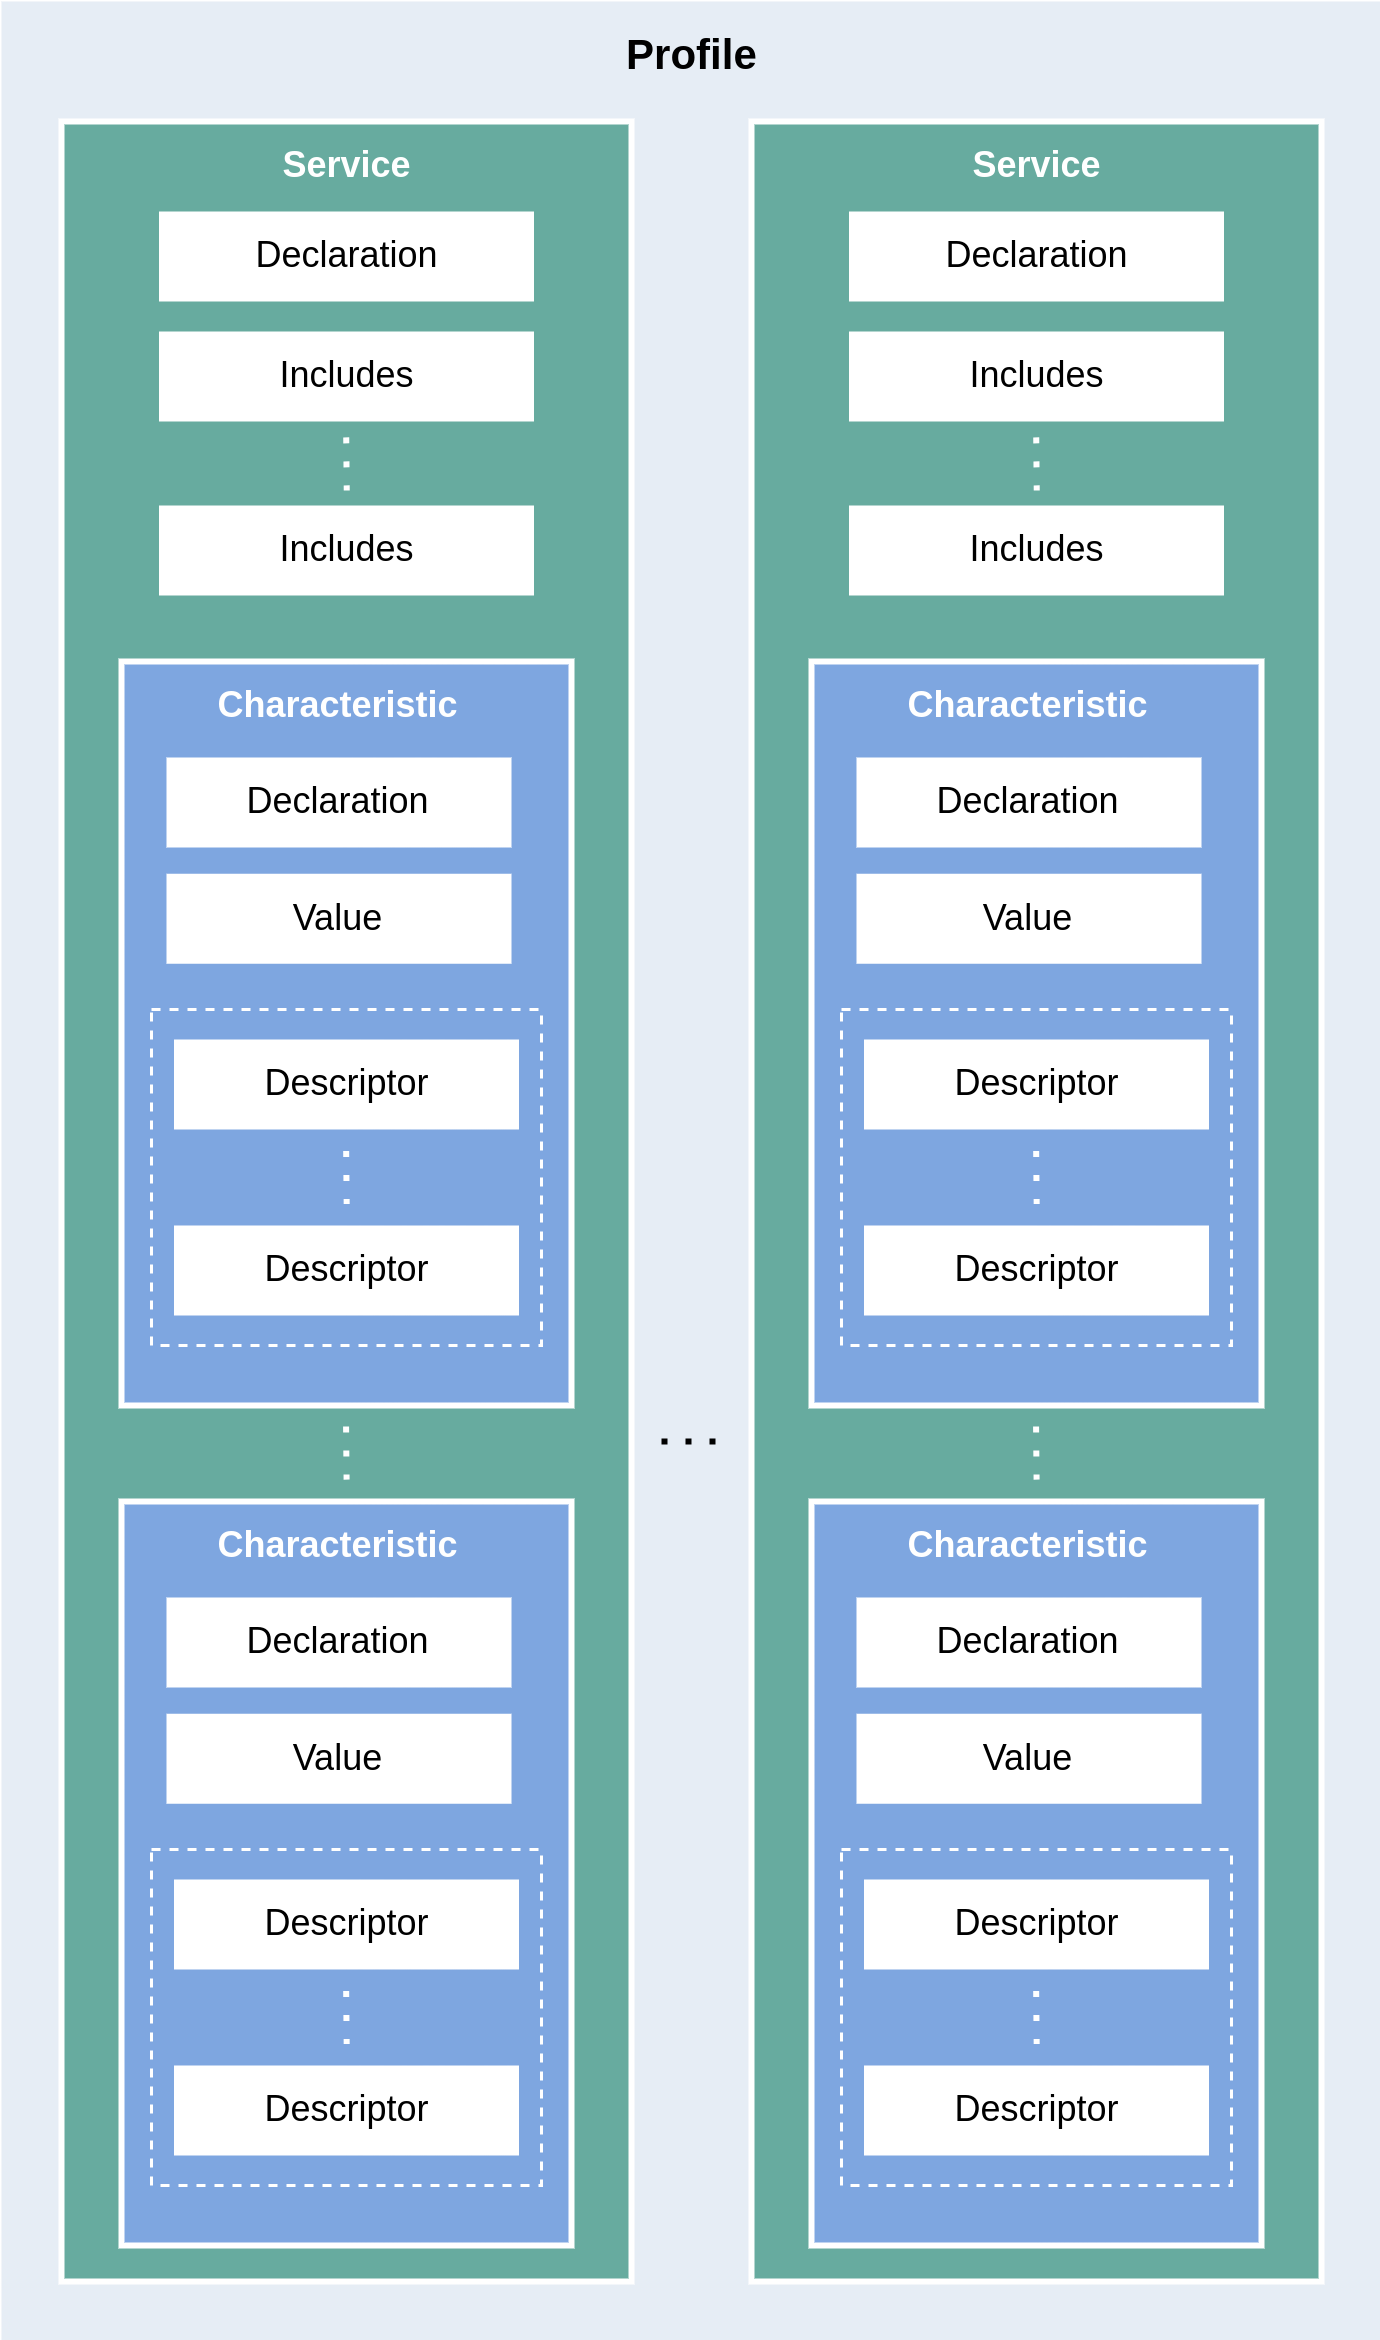
\includegraphics[width=0.5\linewidth]{imagens/ble-gatt-architecture.png}
    \caption{BLE GATT Hierarchical Architecture \cite{gatt}}
    \label{fig:placeholder}
\end{figure}
\vspace{5mm}

In our implementation, the \textit{bluezero} library is used to expose the
Raspberry Pi as a GATT peripheral over the Linux BlueZ stack via D-Bus.
A \texttt{Peripheral} object is configured with a service and its
characteristics, each assigned a Universally Unique Identifier (UUID), 
permission flags, and a callback. For \texttt{notify} characteristics, 
bluezero invokes the \texttt{notify\_callback} once on subscribe and once on 
unsubscribe, passing the live characteristic object. Periodic transmission is 
then driven by a GLib timer that calls \texttt{characteristic.set\_value()} at 
the desired interval, which BlueZ translates into a BLE notification delivered to 
the connected device. The server is started by calling \texttt{peripheral.publish()},
which hands execution to the GLib main loop indefinitely \cite{bluezero}.


\section{Project Synthesis and Differentiation}

In our analysis of the current alternatives to our project, we believe our implementation provides an alternative not seen in any other similar project for several reasons:

\begin{itemize}
    \item \textbf{Open-source:} Most alternatives are are not open-source, which make the modification or modular separation of each of it's components virtually impossible;
    \item \textbf{Modular Components:} Our project is separated in two different modules: Controller and Mobile App. Due to this, our project is flexible to the implementation of different alternatives as long as they are in accordance to the same communication protocol between modules;
    \item \textbf{Database integration:} From our research, every other alternative is a real-time monitoring. Ours gives the possibility of storing all the CAN dataframes in a database for posterior use, such as future simulations or statistical analysis;
    \item \textbf{Cross-plataform Accessibility:} Most options are purely limited to one plataform, be it a computer or a mobile device. Our implementation allows us to monitor the same data in different platforms at the same time, be it computer, mobile device or any other future device with a bluetooth connection;
    \item\textbf{Cheap and easy do aquire hardware:} Many other implementations utilize hard to source components, or may require a difficult setup.
\end{itemize}

Main close competitors to the proposed system:
 
\begin{itemize}
    \item Tuner Studio Dashboard(only dashboard) \cite{ts};
	\item uaDash(only dashboard)\cite{uadash};
	\item MegaLog viewer (only logger)\cite{mlviewer}.
\end{itemize}





\chapter{Implementation}

% !TeX root = ../main.tex
\section{System Architecture}



\begin{figure}[H]
  	\centering   
    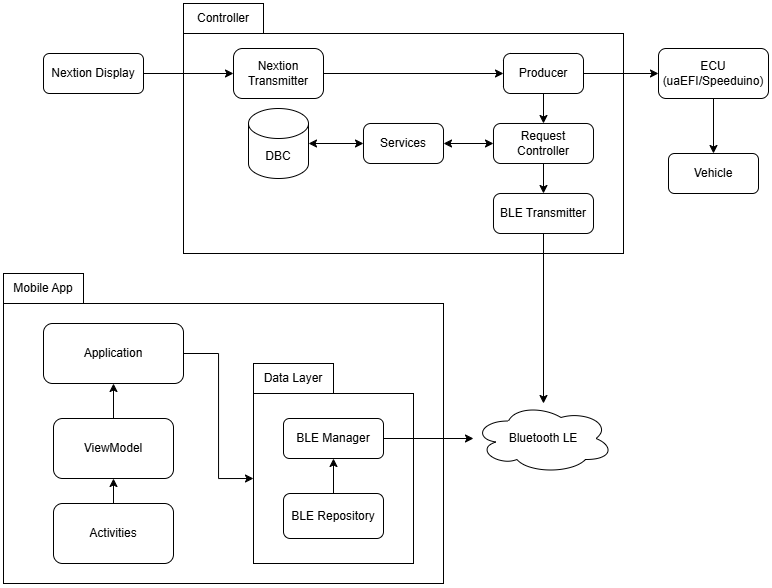
\includegraphics[width=0.8\linewidth]{imagens/project_diagram.png}
    \caption{Project Architecture Diagram}
    \label{fig:prj_arch}
\end{figure}

Figure \ref{fig:prj_arch} illustrates the overall system architecture. The ECU communicates with the Controller via a wired CAN serial link, providing a continuous stream of raw engine frames that are decoded against the vehicle's DBC definition file. At its core sits the Controller, running on the Raspberry Pi Zero 2W, which serves as the central hub for all data acquisition and distribution.  Processed data is simultaneously forwarded to a Nextion display terminal, providing immediate on-site visualisation of critical engine parameters. In parallel, the Controller operates as a Bluetooth Low Energy GATT peripheral, advertising live sensor data to any subscribed central device within range. In the current implementation, an Android mobile application acts as that central, receiving the BLE notifications and presenting the decoded signals in a real-time dashboard. 

\subsection{Controller Configuration File}

The behaviour of the Controller is defined through a JSON configuration file named \texttt{config.json}. This approach separates deployment-specific settings from the application source code, allowing the same software to be adapted to different ECUs, serial interfaces, display devices, and acquisition requirements without modifying its implementation. The file is loaded during application start-up and is also read by the initialization script to determine which hardware interfaces must be available before the Controller is launched.

The \texttt{type} parameter selects the data producer. The value \texttt{rusefi\_can} enables the CAN acquisition path through a GVRET-compatible serial adapter, whereas \texttt{speeduino} \texttt{\_arduino} selects the direct Speeduino serial protocol. The \texttt{mode} parameter selects the local output interface: \texttt{nextion} starts the external Nextion display thread, while \texttt{pi\_screen} starts the PyQt-based interface on a display connected directly to the Raspberry Pi. These parameters allow the acquisition source and the visualization method to be selected independently.

For the \texttt{rusefi\_can} producer, \texttt{com} identifies the serial device associated with the CAN adapter and \texttt{baud\_rate} defines its communication speed. The \texttt{dbc} parameter specifies the path of the DBC file used to translate raw CAN frames into physical vehicle signals. Relative DBC paths are resolved from the Controller directory during start-up. When the \texttt{speeduino\_arduino} producer is selected, the equivalent serial settings are provided through \texttt{port} and \texttt{baudrate}, and \texttt{command} defines the request byte sent to the ECU before each data packet is read. Consequently, only the parameters associated with the selected producer are required during a particular deployment.

Data persistence and diagnostic output are controlled by a separate group of parameters. The \texttt{session\_description} field provides a human-readable description for an acquisition session. The \texttt{state\_save\_interval}, expressed in seconds, determines the minimum interval between consecutive normalized vehicle-state records stored in the database. Raw CAN frames may still be processed at a higher rate, so this value controls database snapshot frequency rather than CAN bus acquisition frequency. The \texttt{log\_can\_activity} flag enables or disables periodic CAN activity messages, while \texttt{can\_log} \texttt{\_interval} determines how frequently the number of received, decoded, and undecoded frames is written to the application log.

The Nextion interface is configured through \texttt{nextion\_port} and \texttt{nextion\_baud}, which define its UART device and communication speed. The \texttt{nextion\_sessions\_interval} parameter determines how frequently the session list is refreshed, and \texttt{nextion\_sessions} \texttt{\_limit} defines the maximum number of sessions presented on the display. The values of \texttt{shift\_point} and \texttt{redline}, both expressed in revolutions per minute, control the RPM visualization: the former determines when the shift indicator changes state, while the latter defines the upper RPM scale used by the dashboard and session graphs.

Finally, \texttt{bluetooth\_enabled} determines whether the BLE server is started together with the Controller. Disabling this option allows acquisition, database storage, and local visualization to continue without exposing the GATT service. The configuration file therefore acts as the central deployment description of the platform, while default values implemented by the software are used for selected optional parameters when they are omitted.

\section{Data Analysis Techniques in Motorsport}
\subsection{Statistical Analysis}

The proposed system records a set of normalized vehicle parameters derived from CAN messages and stored periodically in the database. The currently logged parameters include:

\vspace{-0.2cm}
\begin{table}[H]
\centering
\begin{tabular}{|c|p{12cm}|}
\hline
\textbf{Parameter} & \textbf{Description} \\
\hline

RPM & Engine speed in revolutions per minute, primary indicator of engine operating speed.\\
\hline

SYNC & ECU/engine synchronization status, indicates whether the ECU has valid crankshaft and camshaft position information. \\
\hline

ENGINE & General engine operating status, useful for determining whether the engine is stopped, cranking, or running. \\
\hline

MAP & Intake manifold absolute pressure, one of the primary engine load measurements used for fuel calculations. \\
\hline

BARO & Ambient atmospheric pressure, used for altitude and weather compensation. \\
\hline

TPS & Throttle position, represents driver demand and throttle opening percentage. \\
\hline

IAT & Intake air temperature, affects air density and fueling calculations. \\
\hline

CLT & Engine coolant temperature, critical for warm-up enrichment and engine protection strategies. \\
\hline

AFR & Measured air-to-fuel ratio, key indicator of combustion mixture quality and engine tuning. \\
\hline

EGO & Fuel correction based on oxygen sensor feedback, represents closed-loop fueling adjustments applied by the ECU. \\
\hline

PW & Injector opening duration, directly relates to the amount of fuel delivered to the engine. \\
\hline

VE & Volumetric efficiency used in fuel calculations, represents how effectively the engine fills its cylinders with air. \\
\hline

ADV & Ignition timing advance, major factor of power output, efficiency, and knock resistance. \\
\hline

DWELL & Ignition coil charging time, determines the energy available for spark generation. \\
\hline

BAT & Electrical system voltage, important for injector operation, ignition performance, and system health monitoring. \\
\hline

BOOST & Target boost pressure, desired manifold pressure set by the ECU for forced-induction engines. \\
\hline

DUTY & Wastegate control duty cycle, indicates how aggressively the ECU is controlling boost pressure. \\
\hline

VSS & Vehicle speed, used for logging, speed-based strategies, and traction-related functions. \\
\hline

FAN & Cooling fan status, indicates whether the radiator cooling fan is active. \\
\hline

FP & Fuel pump status, shows whether the ECU has enabled the fuel pump output. \\
\hline

BOOSTCUT & Overboost protection status, indicates whether boost safety limits have been exceeded and protective intervention is active. \\
\hline

\end{tabular}
\caption{ECU Parameters Displayed by the Data Logger}
\label{tab:ecu_parameters}
\end{table}

\section{Hardware development}
\subsection{Hardware schematics}
Our current hardware implementation is comprised of a Raspberry Pi Zero 2W, to which connects a nextion (via serial through the GPIO) and has a USB connection to a GVRET CAN module, which in this case, is a XIAORet, which was also developed in ISEL. \cite{nextion}

The Nextion connection to the raspberry Pi is defined as such:

\begin{figure}[H]
    \centering
    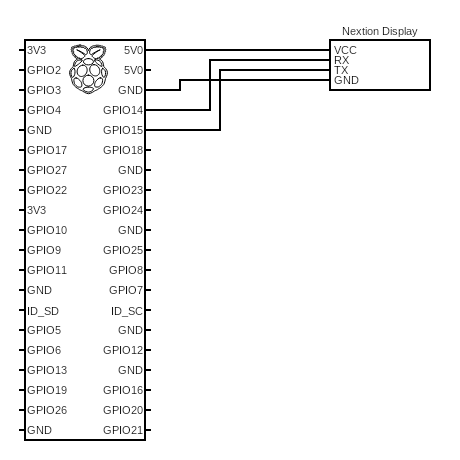
\includegraphics[width=0.5\linewidth]{circuit.png}
    \caption{Electric diagram of the Raspberry Pi and Nextion screen}
    \label{fig:placeholder}
\end{figure}

\subsection{XIAORet comunication protocol}
The XIAORet is a ESP32 microcontroller based CAN Module, that implements the SavvyCan Comunication protocol \cite{savvy}.
SavvyCan is widely used CAN tool for logging, receiving, sending CAN frames and much more. Its widely used in the motorsport world, Formula student and many applications where a CAN tool is needed.
The SavvyCan Comunication protocol is defined as such: 
\begin{itemize}
    \item First, we need enable binary so the following hex command is sent to the XIAORET:0xE7
    \item Secondly, we loop through the received CAN frames, parsing each message. For each frame, the system extracts the timestamp, CAN identifier, data length code (DLC), and payload bytes from the serial stream. The extracted identifier is then processed using a bitmask to ensure compatibility with both standard and extended CAN formats. Subsequently, the frame is matched against the DBC definition, allowing the raw payload to be decoded into meaningful vehicle signals. When a valid mapping is found, the decoded values are integrated into the internal ECU state representation; otherwise, the frame is preserved in its raw form to maintain traceability and support debugging.
\item Although the presented sollution supports 29bit CAN Extended frames, only 11bit CAN Standard frames were tested.
\end{itemize}

\begin{figure}[H]
    \centering
    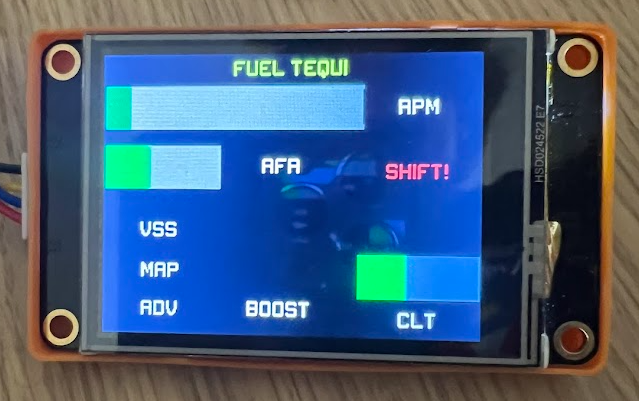
\includegraphics[width=0.5\linewidth]{nextion1.png}
    \caption{Nextion screen 1}
    \label{fig:placeholder}
\end{figure}
\begin{figure}[H]
    \centering
    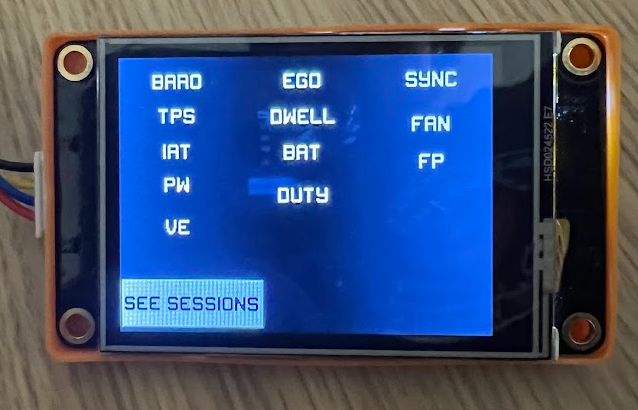
\includegraphics[width=0.5\linewidth]{nextion2.png}
    \caption{Nextion screen 2}
    \label{fig:placeholder}
\end{figure}

\section{Software Implementation}

\subsection{Python Controller}

%\subsubsection{Domain & Repository}

The Python Controller is responsible for several different tasks such as:
\begin{itemize}
    \item \textbf{CAN Connection:} Connection between the ECU module and the Python application using a serial USB link;
    \item \textbf{Database Manager:} Control the database interactions, storing or retrieving the necessary data;
    \item \textbf{UI Display:} Present the information required using a Nextion device, be it real-time from cache or through database requests;
    \item \textbf{Bluetooth Connection and Data Relay:} Connection between the Python application and a connected Bluetooth device (using a mobile app in our implementation).
\end{itemize}

For that end, the application itself has several different inner modules that we will now breakdown and explain, starting with the domain and repository layers.

The \textbf{Domain} and \textbf{Repository} layers are working as a pair since the domain defines the way each data structure is implemented and the repository defines how it gets stored and retrieved. Neither are responsible for the restriction logic - that will be the responsibility of \textit{Services}.

\begin{figure}[H]
    \centering
    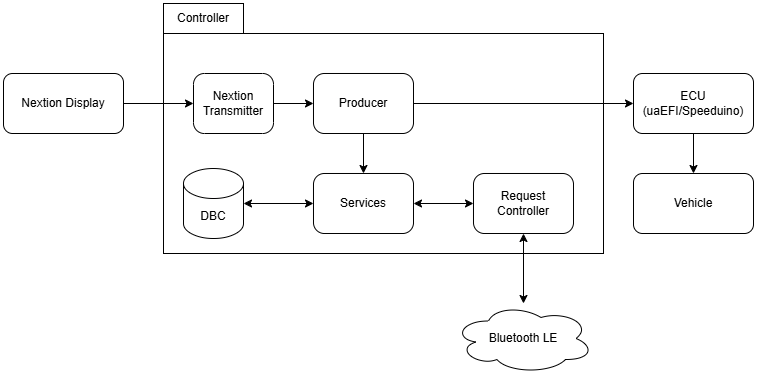
\includegraphics[width=0.8\linewidth]{imagens/controller_diagram.png}
    \caption{Controller Structure Diagram}
    \label{fig:placeholder}
\end{figure}

The domain consists of four different types of classes - \texttt{Session}, \texttt{CANFrame}, \texttt{Signal} and \texttt{VehiculeState} - each used simply to keep information that is either being retrieved or stored in the database.

 A session represents one continuous recording period with a start timestamp, an optional end timestamp that begins as None, and a human-readable description. A \texttt{CANFrame} captures a single raw message off the bus: which session it belongs to, when it arrived, the CAN arbitration ID, the data length code, and the raw data bytes as a string. A Signal is the decoded output of a frame, associating a signal name and its parsed numeric value and unit back to the frame it came from. A \texttt{VehicularState} records the current dataframe state of the vehicle for easy access to the complete information of the vehicle in a specific timestamp. Each domain class has it's respective repository class that will handle the requests to the database.

The repository layer sits directly on top of SQLite database and mirrors that domain structure previously stated. Each repository module opens its own connection to the database at each request and automatically closes said connection when the request is finished using a \texttt{with closing(...)}. This also means that any cross-table operation that needs to be atomic, such as inserting a frame and its signals together, has no transaction boundary protecting it, since each call commits independently. That is an architectural limitation worth addressing before the project handles high-frequency acquisition in production

The services module acts as the single entry point through which the rest of the application interacts with the database. Rather than letting the acquisition pipeline, the UI, or any other consumer reach into a repository directly, everything that needs to read or write persistent data goes through here. In practice every function in the module is a one-liner that receives arguments, forwards them to the appropriate repository function, and returns whatever the repository gives back. The value of this pattern is not in the logic it adds — there is none — but in the boundary it creates: if a repository is ever renamed, replaced, or refactored, only this file needs to change.

We have a class \texttt{SignalCache} that will be the singleton class that will record and transmit the latest dataframe obtain from the ECU and relay it to both the UI Display and the Bluetooth transmission for a faster access to the real-time information.

The BLE transmitter, our bluetooth layer, turns the device into a BLE GATT that an android device is able to discover, connect to and subscribe to continuos sensor data acquired by the ECU. For it's proper operation, we create an instance of \textit{BLETlmServer}, which will build the GATT tree by creating a \texttt{Peripheral} object bound by the device's Bluetooth adapter MAC address and advertising under the local name "\textit{Vehicular\_Monitor}" and will register one primary service and three characteristics under that service. The first characteristic will be configured with both \texttt{read} and \texttt{notify} flags in order for the mobile client to either poll the data explicitly or to be notified of any updates to the signal cache. This way we can attach two different callback: \texttt{read\_callback} and \texttt{notify\_callback}. The second characteristic will be configured with \texttt{write} flag in order to obtain session requests from the mobile client and has a \texttt{\_session\_request\_cb} as a \texttt{write\_callback}. This characteristic exists to be able to accurately send requested information through the third characteristic. The third characteristic is similar to the first one with different callbacks: \texttt{\_session\_response\_read\_cb} and \texttt{\_session\_response\_notify\_cb}

The notify mechanism is the most important part to understand correctly. In \textit{Bluezero}, \texttt{notify-callback} is not a function that gets called each time a notification needs to be sent — it is a status callback that fires once when a client subscribes and once when it unsubscribes. When it fires with \texttt{notifying=True}, the callback receives a reference to the live characteristic object and immediately schedules a repeating GLib timer set to fire every 200 milliseconds. Each time the timer fires, \texttt{\_send\_notify} calls \texttt{characteristic.set\_value()} with the latest encoded cache string, which emits a D-Bus \texttt{PropertiesChanged} signal that BlueZ translates into an actual BLE notification packet sent to the Android device. The timer returns True on every successful call to keep itself alive, and only returns False — which removes it — if the characteristic reference has been cleared. When the client unsubscribes and notify\_cb fires with notifying=False, the stored characteristic reference is cleared and the GLib timer is cancelled with GLib.source\_remove, stopping all further transmissions until a new subscription arrives.

As mentioned before, the BLE transmitter utilizes two characteristics in charge of obtaining session requests and returning session responses towards the remote device. These characteristics allow the use of several different commands: the session list (format: \texttt{"GET\_SESSIONS"}), session information by identifier (format: \texttt{"GET\_SESSION:\_ID\_"} ), session creation (format: \texttt{"CREATE\_SESSION"}), and session ender (format: \texttt{"END\_SESSION"}). These commands either return a list of values obtained from the database, or a boolean in case of error, and are available to any application that is connected to the available service provided by the python controller and is connected through BLE. 

Calling start() triggers ble.publish(), which begins advertising the peripheral and hands control to the GLib main loop. This call never returns under normal operation — everything that needs to happen alongside the BLE server, such as the mock data generator or the console status printer, must be running in daemon threads before start() is called. The process must also be launched with \textit{sudo ./venv/bin/python3} rather than bare sudo python3, because BlueZ requires root privileges and the system Python does not have bluezero installed.

\subsection{Python Producer}

The Python producer application constitutes the core of the proposed CAN platform controller, being responsible for data acquisition, processing, storage, and visualization. The system is implemented in Python and follows a modular, multi-threaded architecture designed to ensure high performance, scalability, and maintainability. Both the controller are integrated and running in the same processor as a way to not only obtain all necessary information through the producer and implement all required functionality through the controller.

From an architectural perspective, the application adopts a distributed processing model based on multiple worker threads. This approach allows different responsibilities such as data acquisition, decoding, persistence, and visualization to be executed concurrently. As a result, the system minimizes bottlenecks and ensures real-time responsiveness when handling high-frequency CAN data streams.

The application entry point is defined in \textit{main.py}, which orchestrates the system initialization workflow. At startup, the application reads a configuration file (\textit{config.json}) that defines both the data source (\textit{producer type}) and the output interface (\textit{mode}). This configuration-driven design enables flexibility, allowing the same software to operate with different ECUs and visualization methods without requiring code modifications.

Following configuration loading, the system initializes the SQLite database (\textit{ecu\_data.db}) and ensures that all required tables are created. These include tables for raw CAN frames, acquisition sessions, and normalized vehicle state snapshots. The database layer is abstracted through a repository pattern, which decouples data persistence from the rest of the application logic and improves maintainability.


\begin{figure}[H]
    \centering
    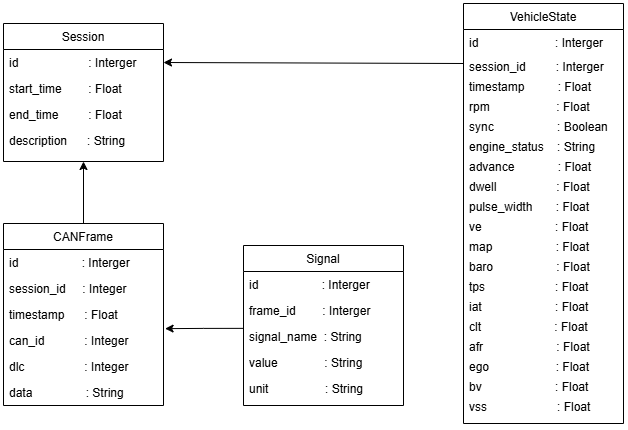
\includegraphics[width=0.7\linewidth]{imagens/db_diagram.png}
    \caption{Database Diagram}
    \label{fig:placeholder}
\end{figure}

The data acquisition process is handled by a dedicated producer thread, which can operate in different modes depending on the selected ECU interface. In the \textit{rusefi\_can} mode, the system reads CAN frames via a SavvyCan-compatible serial adapter. These frames are decoded using a DBC file, allowing raw binary messages to be translated into meaningful automotive signals. Alternatively, in the \textit{speeduino\_arduino} mode, the application directly parses structured serial data packets via USB, from the Speeduino ECU.

Decoded signals are then mapped into a unified internal representation of the vehicle state. This state is maintained in a shared memory structure called \textit{signal\_cache}, which always stores the most recent values received from the ECU. This design avoids repeated database queries and enables fast access for visualization components.

In parallel with the acquisition process, additional threads handle data persistence and output. The system periodically stores snapshots of the vehicle state in the database, enabling offline analysis while retaining the raw CAN traffic required for traceability.

\subsubsection{CAN Data Persistence and Session Recording}

Database recording is organized around acquisition sessions. The Controller continues to acquire and decode CAN traffic immediately after start-up, but persistent recording only begins when a session has been created. In the present Nextion workflow, the display starts a session by transmitting a \texttt{NEW\_SESSION} request. If another session is already active, its end timestamp is recorded before a new row is inserted into the \texttt{sessions} table. Each subsequent database record is associated with the identifier of the active session. Before this request is received, decoded data remains available to the live display and Bluetooth interface through the signal cache, but it is not written to the session tables.

Two complementary forms of data are stored during a session. First, every valid GVRET CAN frame is inserted into the \texttt{can\_frames} table, including frames whose identifiers are absent from the DBC file or whose payload cannot be mapped to the normalized vehicle state. Each row contains the session identifier, reception timestamp, CAN identifier, data length code, and hexadecimal payload. This provides a complete record of the received bus traffic and preserves undecoded frames for subsequent inspection or reprocessing. The current implementation performs and commits each insertion individually rather than grouping several frames into a transaction.

Second, decoded frames update an in-memory aggregate containing the latest known value of every supported vehicle parameter. Since the RusEFI base messages distribute related signals across several CAN identifiers, an individual decoded frame generally modifies only part of this aggregate. For example, one message updates engine speed, ignition advance, and vehicle speed, while another updates manifold pressure and temperatures. Values obtained from earlier messages are retained until they are replaced, allowing the aggregate to represent the most recent complete vehicle state.

A copy of this aggregate is periodically inserted into the \texttt{vehicle\_state} table. The minimum interval between consecutive snapshots is defined by the \texttt{state\_save\_interval} configuration parameter, expressed in seconds. With a value of \texttt{1.0}, the system records approximately one vehicle-state row per second; values of \texttt{0.5} and \texttt{0.25} allow maximum rates of approximately 2 and 4~Hz, respectively. The interval is evaluated when a decoded frame arrives, rather than by an independent timer. Consequently, a snapshot is written on the first decoded frame received after the configured interval has elapsed. No state is stored during periods in which no decodable traffic is received, and the actual spacing may therefore be slightly greater than the configured value.

The snapshot interval is reset whenever the active session changes, causing the first decoded frame of a new session to be recorded immediately. Each \texttt{vehicle\_state} row contains the session identifier, insertion timestamp, and the complete normalized set of engine, load, temperature, fuelling, ignition, electrical, boost, speed, and status parameters. Its timestamp is generated by the Raspberry Pi at insertion time. By contrast, raw CAN frame rows use the frame reception time captured by the acquisition process. The adapter-provided GVRET timestamp is used during parsing but is not presently persisted as a separate database field.

This separation provides different resolutions for different purposes. The \texttt{can\_frames} table follows the incoming bus rate and maintains the detailed source record, whereas \texttt{vehicle\_state} contains a lower-frequency time series suitable for session graphs and general analysis. For example, a ten-minute session with a snapshot interval of one second produces approximately 600 vehicle-state rows, while the number of raw frame rows depends directly on CAN traffic and may be several orders of magnitude higher. Session graph requests query \texttt{vehicle\_state}, filter rows by session identifier, and order them by timestamp before the selected parameters are plotted.

The database schema also contains a \texttt{signals} table intended to associate individually decoded values with their source CAN frames. This table is supported by the repository layer but is not populated by the current GVRET acquisition path; normalized values are instead retained through the periodic \texttt{vehicle\_state} snapshots. Furthermore, equivalent persistence has not yet been integrated into the \texttt{speeduino\_arduino} reader, which currently updates the live signal cache without creating raw-frame or vehicle-state records. These constraints define the present recording scope and identify areas for future development, particularly transaction batching, explicit session termination during shutdown, and a common persistence path for both supported producers.

For visualization, the application supports two independent output modes. In the \textit{Nextion} mode, a dedicated thread continuously reads the latest values from the \textit{signal\_cache} and transmits them over a serial interface to a Nextion display, providing a lightweight, embedded graphical interface. In the \textit{pi\_screen} mode, a PyQt-based dashboard runs locally on the Raspberry Pi, periodically refreshing the displayed values using a timer mechanism. The separation between data acquisition and visualization ensures that user interface performance does not interfere with real-time data processing.

\subsubsection{Nextion Session Graph Generation}

In addition to displaying live values, the Nextion interface can plot signals stored during a previous acquisition session. A graph request issued by the display identifies the selected session and the signals to be represented. The Controller resolves the displayed session index to its database identifier, retrieves the corresponding vehicle-state records, and converts the resulting series into native Nextion drawing commands. The graph is therefore rendered by the display itself using line, fill, and text commands, without transferring a bitmap or relying on the Nextion waveform component.

The plotting area begins at coordinate $(35,45)$ and has a width of 410 pixels and a height of 170 pixels. Samples are distributed uniformly along the horizontal axis, from $x=35$ to $x=445$, according to their order in the retrieved series. For a series containing $N$ samples, the horizontal coordinate of sample $i$ is given by

\begin{equation}
x_i = 35 + \left\lfloor \frac{i}{N-1} \times 410 \right\rfloor .
\end{equation}

This representation assumes that stored vehicle-state samples are separated by approximately regular intervals. When a session contains more than 410 records, the series is reduced to 410 uniformly selected samples. Both endpoints are retained, ensuring that the complete session is represented while limiting the number of serial commands and avoiding multiple samples being assigned to the same horizontal pixel.

Each signal is normalized independently on the vertical axis using a predefined physical range. If $v_i$ is the measured value, and $v_{\min}$ and $v_{\max}$ are the limits assigned to that signal, its vertical coordinate is calculated as

\begin{equation}
y_i = 45 + 170 - \left\lfloor
\frac{v_i-v_{\min}}{v_{\max}-v_{\min}} \times 170
\right\rfloor .
\end{equation}

Values outside the specified range are clamped to the upper or lower graph boundary. The inversion in this expression is required because the Nextion coordinate system places the origin at the top-left corner of the screen. Consequently, a signal's minimum value is plotted at $y=215$, its midpoint at approximately $y=130$, and its maximum at $y=45$.

The ranges used by the implementation are listed in Table~\ref{tab:nextion_graph_ranges}. The RPM upper limit is obtained from the configurable \texttt{redline} value; the remaining limits are fixed according to the expected operating range of each parameter.

\begin{table}[H]
\centering
\begin{tabular}{|l|c|c|l|}
\hline
\textbf{Signal} & \textbf{Minimum} & \textbf{Maximum} & \textbf{Unit} \\
\hline
Engine speed (RPM) & 0 & \texttt{redline} & rpm \\
Air--fuel ratio (AFR) & 10 & 20 & -- \\
Coolant temperature (CLT) & 0 & 120 & $^{\circ}$C \\
Intake air temperature (IAT) & 0 & 80 & $^{\circ}$C \\
Throttle position (TPS) & 0 & 100 & \% \\
Manifold pressure (MAP) & 0 & 250 & kPa \\
Barometric pressure (BARO) & 80 & 120 & kPa \\
Ignition advance (ADV) & $-20$ & 60 & degree \\
Injector pulse width (PW) & 0 & 20 & ms \\
Battery voltage (BAT) & 0 & 16 & V \\
Boost target & 0 & 250 & kPa \\
Boost duty & 0 & 100 & \% \\
Vehicle speed (VSS) & 0 & 250 & km/h \\
\hline
\end{tabular}
\caption{Vertical scales used for Nextion session graphs}
\label{tab:nextion_graph_ranges}
\end{table}

After coordinate conversion, consecutive points belonging to the same signal are joined by line commands. Up to six signals can be distinguished using the predefined red, blue, green, orange, cyan, and magenta sequence; colours are reused if additional signals are requested. Since every signal uses its own vertical scale, overlapping curves indicate a similar relative position within their respective operating ranges rather than equality of their physical values. This normalization allows parameters with different units and magnitudes, such as RPM, AFR, and coolant temperature, to be inspected together within the limited display area.

To support deployment as an embedded system, the application includes an initialization script (\textit{init.sh}) designed to be executed as a systemd service (or first time startup). This script prepares the runtime environment, waits for required hardware interfaces (such as serial devices), and guarantees automatic startup and recovery in case of failure. This makes the system robust and suitable for unattended operation in automotive environments.

Overall, the combination of a multi-threaded architecture, modular design, configuration-driven behavior, and efficient data handling mechanisms allows the Raspberry Pi application to meet the real-time requirements of vehicular data acquisition systems while maintaining flexibility and extensibility for future developments.

\clearpage
\subsection{Android application}

The Android application is utilized as an exterior module to the Python Controller that will receive data via BLE from the controller and display it in an intuitive manner. This module could be replaced for any other application as long as it follows the communication protocol defined by the controller and be connected to the controller via Bluetooth.

\begin{figure}[H]
    \centering
    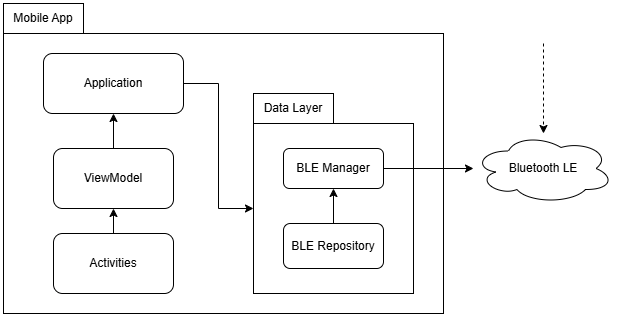
\includegraphics[width=0.8\linewidth]{imagens/mobile_diagram.png}
    \caption{Mobile Application Structure Diagram}
    \label{fig:placeholder}
\end{figure}

The structure of the Android application is as follows:
\begin{itemize}
    \item \textbf{Application:} Root of the entire dependency structure and implements the \texttt{Dependency Container} interface that declares three different singletons - \texttt{Ble Manager}, \texttt{Ble Repository} and \texttt{BleViewModelFactory} - available to the rest of the application
    \item  \textbf{Activity:} All activities extend \texttt{BaseActivity} and are the boundary between the application and it's UI. \texttt{BaseActivity} standardizes lifecycle logging across every screen and exposes a generic \texttt{navigate<T>()} helper used to move between activities, as well as a {backPressed()/backAware()} hook for consistent back-navigation handling. The \texttt{MenuActivity} is the primary activity. It manages the application permissions (\texttt{BLUETOOTH\_SCAN} and \texttt{BLUETOOTH\_CONNECT} and \texttt{ACCESS\_FINE\_LOCATION}) and starts the scanning for connected Bluetooth devices, working as a link to distribute said Bluetooth device's information to the rest of the possible activities. Selecting a scanned device opens \texttt{DeviceMenuActivity}, a per-device menu (Live Data, Sessions Information, Overall Statistics, Device Information) that in turn opens \texttt{DataDisplayActivity} to show the live data stream for that device. \texttt{AboutActivity} is reachable from \texttt{MenuActivity} and shows application information.
    \item \textbf{ViewModel:} The core of the application's state management through \texttt{BleViewModel}. It holds the current state \texttt{\_uiState} of the current application and exposes it in a immutable \textit{StateFlow} to the current observable screen. When \texttt{.start()} is called, it launches a coroutine that collects cvs strings from \texttt{BleRepository.canData} and when \texttt{.connect()} is called it passes the selected device to the repository to initiate GATT connection. Each incoming csv line is parsed by \texttt{parseCanData()} into a \texttt{MainUiState} carrying the individual channels reported by the controller (RPM, coolant temperature, AFR, TPS, MAP, battery voltage, dwell, ignition timing, VSS, IAT, EGO correction, VE, and sync status), with the raw string preserved alongside the parsed fields. For development and demonstration without a physical controller connected, \texttt{BleViewModel} also exposes \texttt{.startMockData()}, which generates a continuous stream of plausible randomized values into the same uiState so the UI can be exercised standalone. \texttt{BleViewModelFactory} allows the construction of a \texttt{BleViewModel} with the \texttt{BleRepository} constructor.
    \item \textbf{Model:} The \texttt{BleManager} owns every interaction with the Android Bluetooth stack, scanning for devices, loading already-paired (bonded) devices, and connecting over GATT using a service and three different characteristics that forms part of the defined communication protocol with the controller. \texttt{BleRepository} wraps \texttt{BleManager} as a stable boundary. It re-exposes \texttt{devicesFlow} and \texttt{dataFlow} as \texttt{scannedDevices} and \texttt{canData} respectively, and delegates \texttt{startScan} and \texttt{connectToDevice} directly. Its presence means the \texttt{ViewModel} layer imports nothing from \texttt{BleManager} directly, and the BLE implementation could be replaced or mocked entirely without touching a single \texttt{ViewModel}.
\end{itemize}


\chapter{Results and validation}

This chapter presents the validation of the platform across two test
environments: Bench and Vehicle, followed by a dedicated
verification of the mobile application and a synthesis of the overall results. 
\par For this validation, the experimental hardware utilized is the following:
\begin{itemize}
    \item uaEFI Ultra Affordable EFI\cite{rusefi_website}
    \item Raspberry Pi Zero 2W (with headers) \cite{raspizero2w}
    \item Motorola G15 \cite{motog15}
\end{itemize}

\vspace{5mm}
\begin{figure}[H]
    \centering
    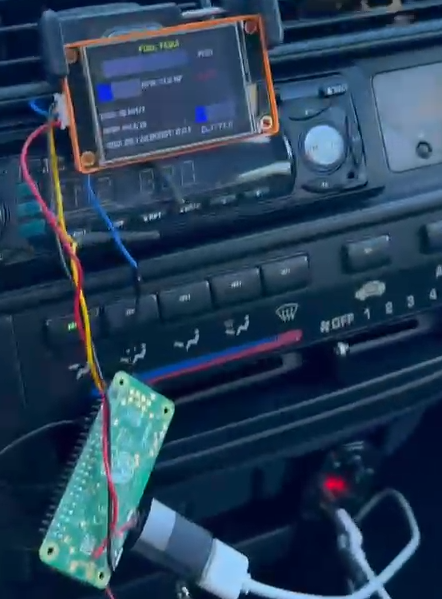
\includegraphics[width=0.35\linewidth]{imagens/hardware_photo.png}
    \caption{Hardware utilized}
    \label{fig:placeholder}
\end{figure}
\vspace{5mm}


\section{Bench Validation}

Bench validation was performed with the Raspberry Pi connected via USB serial
to a Speeduino ECU running on a static test bench, before any vehicle
integration. Each software module was verified in isolation and as part of the
integrated pipeline.
No bench validation was performed with a RusEFI ECU due to testing constraints.

The CAN acquisition pipeline was confirmed to correctly decode all signals
defined in the DBC file, including RPM, coolant temperature, MAP, TPS, AFR,
ignition advance, dwell, and battery voltage. Decoded values were cross-checked
against the reference values programmed into the ECU, with no decoding errors
observed over a 30-minute continuous run.

The \texttt{SignalCache} singleton was verified for thread-safety under
concurrent producer and consumer access. The alias synchronisation mechanism
was also validated, confirming that updates to canonical keys such as
\texttt{clt} and \texttt{advance} were correctly reflected in their aliases
\texttt{temp} and \texttt{timing}.

Database persistence was validated through a complete session lifecycle:
creation, continuous frame and signal insertion over 10 minutes, and
termination. All records were confirmed intact, and session retrieval queries
returned results in the correct order.

The BLE stack was validated using \texttt{test\_ble\_transmitter.py}, which
populated the signal cache with mock sensor data at 5~Hz and transmitted it
to the Android device. Notifications arrived at the expected 200~ms interval
with all 13 payload fields correctly received across a 20-minute streaming
session.


\section{Vehicle Validation}

Vehicle validation was performed on a road vehicle equipped with a RusEFI
ECU. The Raspberry Pi was mounted in the cabin with a CAN connection to the
ECU serial output.

Signal values from the platform were compared against TunerStudio running
simultaneously on a laptop connected to the same ECU. RPM readings matched
within $\pm$5~RPM at stable engine speeds. Coolant temperature correctly
tracked the warm-up curve from cold start to operating temperature. AFR and
EGO correction values were consistent with the closed-loop behaviour visible
in TunerStudio.

A 5-minute driving session produced approximately 5000 CAN frames stored
without write errors or data loss. Session timestamps correctly delimited the
recording window. No crashes, BLE disconnections, or process restarts were
observed throughout. CPU utilisation remained below 60\% across all concurrent
tasks.

\section{Mobile Application Verification}

The Android application was verified in three modes: mock device, bench BLE,
and vehicle BLE.

Device discovery correctly distinguished between paired-only and actively
advertising peripherals, with paired-only device cards rendered as
non-interactable. All 13 sensor fields updated correctly at 5~Hz in the live
data screen. Displayed values were validated against the bench test harness
console output and against TunerStudio during vehicle testing, with no parsing
errors or field misalignments observed.

\vspace{5mm}
\begin{figure}[H]
    \centering
    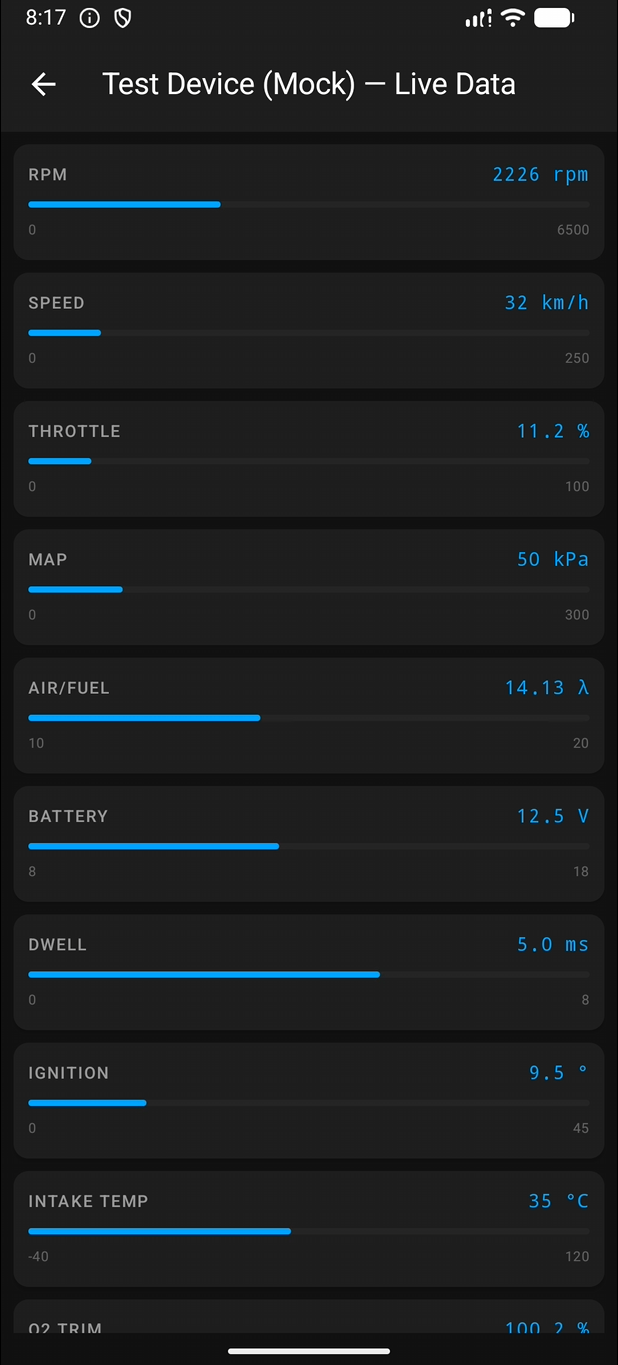
\includegraphics[width=0.35\linewidth]{imagens/mobile_test1.png}
    \caption{Live data display}
    \label{fig:placeholder}
\end{figure}
\vspace{5mm}

\clearpage
Session acquisition and start time recording were verified to be accurate,
with each driving session correctly created and timestamped upon data
collection. The session-specific statistics presented by the application were
confirmed to match the corresponding values stored in the database, indicating
that data acquisition, storage, and retrieval operated correctly throughout the
testing process.

\vspace{5mm}
\begin{figure}[H]
    \centering

    \begin{subfigure}[H]{0.35\textwidth}
        \centering
        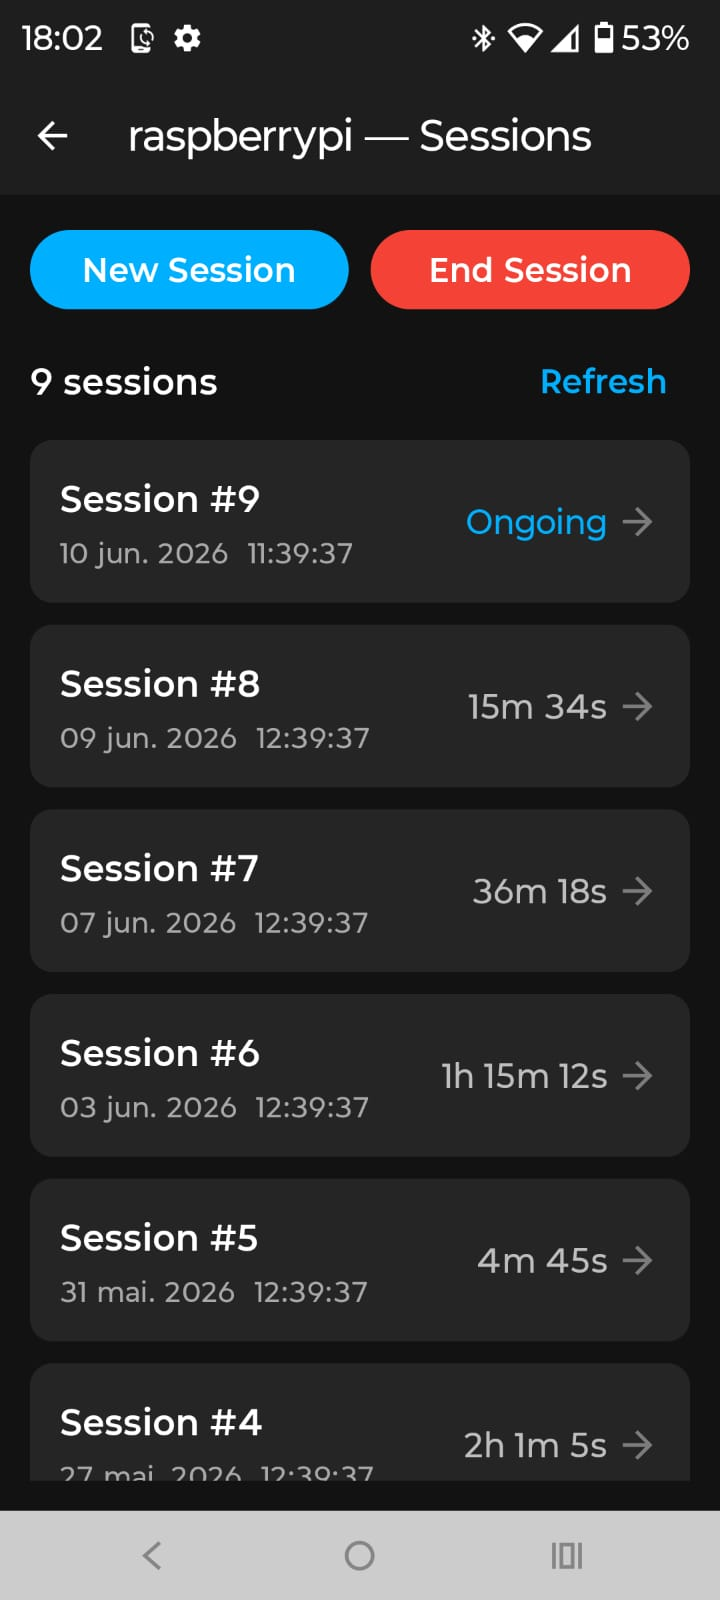
\includegraphics[width=\linewidth]{imagens/mobile_test2.png}
        \caption{Sessions display}
        \label{fig:dashboard1}
    \end{subfigure}
    \hspace{20mm}
    \begin{subfigure}[H]{0.35\textwidth}
        \centering
        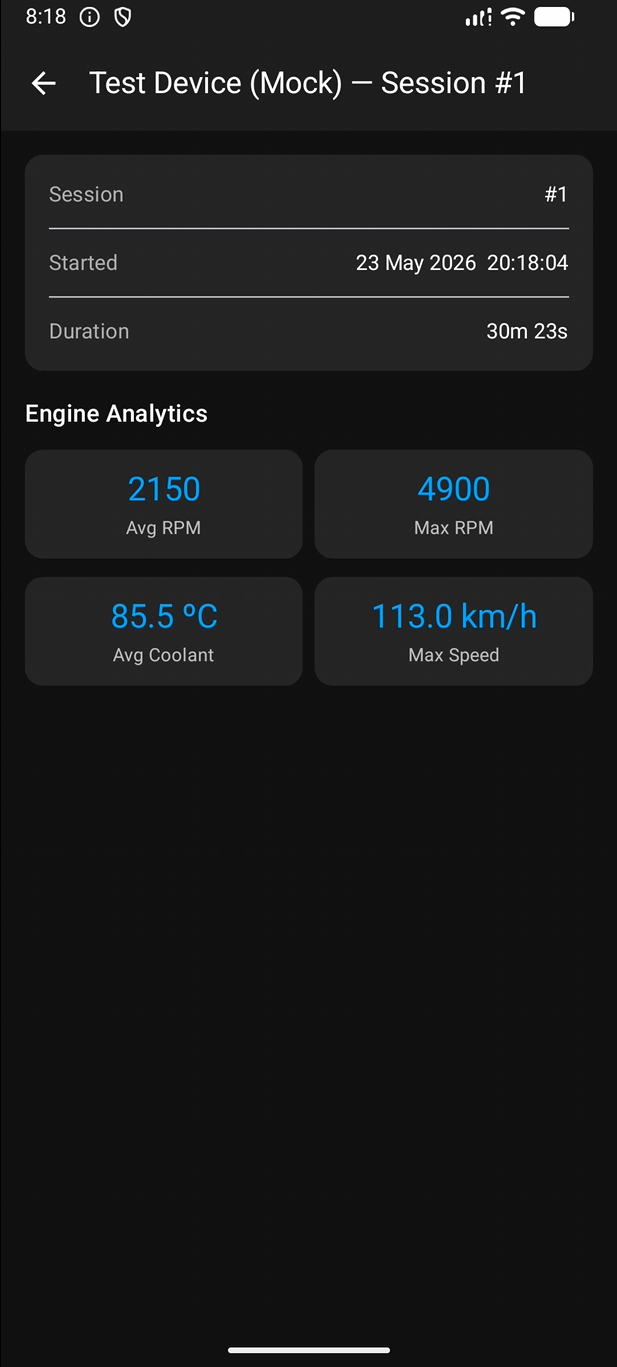
\includegraphics[width=\linewidth]{imagens/mobile_test3.png}
        \caption{Session information display}
        \label{fig:dashboard2}
    \end{subfigure}
    \caption{Session displays}
    \label{fig:dashboards}
\end{figure}
\vspace{5mm}

\clearpage

The overall statistics screen was also validated by comparing its aggregated
values with the complete set of session records stored in the database. The
application consistently displayed accurate cumulative statistics, confirming
the correctness of the aggregation logic and the integrity of the stored data.

\vspace{5mm}
\begin{figure}[H]
    \centering
    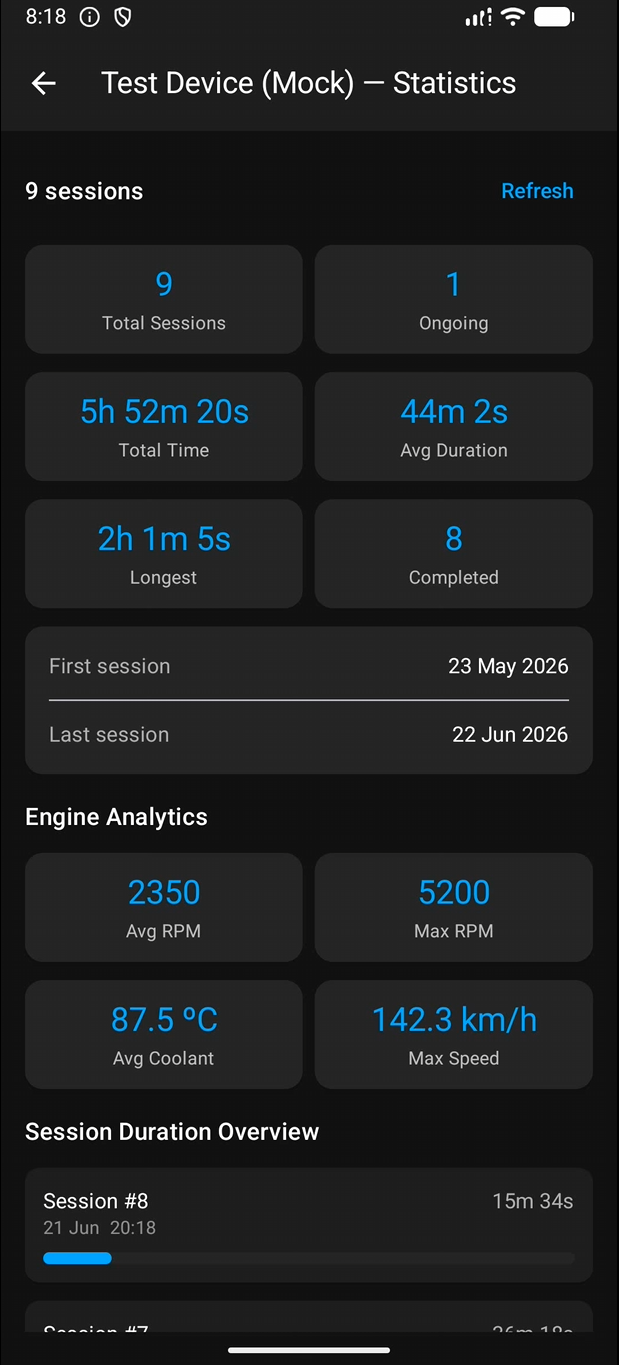
\includegraphics[width=0.35\linewidth]{imagens/mobile_test4.png}
    \caption{Overall statistics display}
    \label{fig:placeholder}
\end{figure}
\vspace{5mm}

\section{Raspberry Pi/Nextion Application verification}

The Raspberry Pi/Nextion interface was verified using both simulated and live
engine data to evaluate communication reliability, display accuracy, and user
interaction. The Nextion display was connected directly to the Raspberry Pi via
UART, while telemetry data was obtained from the shared \texttt{SignalCache}
used by the remaining platform components.

Displayed values, including RPM, coolant temperature, AFR, battery voltage,
manifold pressure, ignition timing, and throttle position, were compared
against the simulated data send or information seen on TunerStudio. All monitored 
signals were updated correctly with no observable inconsistencies between the 
displayed and transmitted data.

Screen navigation and touch interactions were validated across all available
pages. User inputs were correctly interpreted by the Raspberry Pi application,
and page transitions occurred without delays or communication errors. Extended
runtime testing was performed over a continuous 30-minute session, during which
no freezes, application crashes, or UART communication failures were observed.

The refresh rate was sufficient to provide smooth real-time feedback while
maintaining relatively low CPU utilisation on the Raspberry Pi. Throughout vehicle
operation, sensor values remained responsive to engine speed and load changes,
confirming the suitability of the interface for real-time driver monitoring.

Overall, the Raspberry Pi/Nextion subsystem operated reliably and provided an
accurate representation of the acquired ECU data, validating its integration
within the proposed platform.

\section{Results Summary}

Validation confirmed that the platform meets its primary objectives. 
CAN acquisition and DBC-based decoding operated correctly under real 
engine conditions. Continuous datalogging handled
high-frequency writes without data loss. BLE transmission reliably delivered
a 13-signal payload at 5~Hz, and the mobile application correctly displayed
all fields.

The main limitation identified is the absence of automatic BLE reconnection
logic on both the controller and the Android client, currently requiring
manual intervention after an unexpected disconnection. This is the primary
target for improvement in future iterations of the platform.





\chapter{Conclusions}
This work presented a CAN-based data acquisition system implemented on a Raspberry Pi, combining real-time frame acquisition, DBC-based decoding, and structured data storage. The system demonstrates that it is possible to build a functional telemetry platform using low-cost hardware, while maintaining sufficient performance for typical automotive monitoring tasks.

However, several limitations are evident. The current architecture does not enforce strict real-time guarantees, as Python threading and the underlying operating system scheduling can introduce non-deterministic delays. This limits the system's suitability for safety-critical applications.

The abstraction of CAN data into a normalized vehicle state simplifies usage but also reduces flexibility, since only a subset of signals is retained. Any changes to the monitored parameters require modifications in multiple components, including decoding logic and database schema, which impacts maintainability. Furthermore, the system does not currently distinguish between standard and extended CAN frames at a semantic level, which may be relevant in more complex network configurations.

From a data analysis perspective, the platform focuses on acquisition and storage, with limited built-in analytical capabilities. While it enables offline analysis, it does not yet exploit advanced techniques such as anomaly detection, correlation analysis, or predictive models. As a result, much of the potential value of the collected data remains unexplored.

Despite these constraints, the system provides a solid foundation for telemetry in non-critical environments such as entusiast motorsports and Formula Student. It enables consistent data collection, supports debugging and performance evaluation, and improves visibility over ECU behaviour. Future work should focus on improving data throughput, introducing more robust real-time handling, and extending the analytical capabilities of the platform.


\nocite{*}
\typeout{}
\printbibliography 

\end{document}